\documentclass[conference]{IEEEtran}
\IEEEoverridecommandlockouts

\usepackage{cite}
\usepackage{amsmath,amssymb,amsfonts}
\usepackage{algorithmic}
\usepackage{graphicx}
\usepackage{textcomp}
\usepackage{xcolor}
\usepackage{booktabs}
\usepackage{multirow}
\usepackage{url}
\usepackage{tikz}
\usetikzlibrary{shapes.geometric, arrows.meta, positioning, calc, fit, backgrounds}

\begin{document}

\title{Automated Semantic Resume Screening and IT Job Role Classification}

\author{
    \IEEEauthorblockN{
        D. T. D. Perera\IEEEauthorrefmark{1},
        Dulnith K. D.\IEEEauthorrefmark{2},
        K. G. Savinda N. Perera\IEEEauthorrefmark{3}, and
        Yenura S. Karunanayaka\IEEEauthorrefmark{4}
    }
    \IEEEauthorblockA{
        Faculty of Computing, Sri Lanka Institute of Information Technology (SLIIT), Malabe, Sri Lanka\\
        Email: \IEEEauthorrefmark{1}it22089236@my.sliit.lk (ID: IT22089236),
               \IEEEauthorrefmark{2}it22094872@my.sliit.lk (ID: IT22094872),\\
               \IEEEauthorrefmark{3}it22027610@my.sliit.lk (ID: IT22027610),
               \IEEEauthorrefmark{4}it22306272@my.sliit.lk (ID: IT22306272)
    }
}

\maketitle

\begin{abstract}
Automated curriculum vitae (CV) screening in technical recruitment frequently fails due to superficial keyword matching, vulnerability to template artifacts, and crude aggregation of disparate candidate qualifications. In this paper, we present the design and empirical evaluation of Component 1 of the RecruitAI ecosystem: an automated semantic resume screening and job role classification microservice. The system processes heterogeneous PDF/DOCX resumes, applies regularized semantic section detection, and extracts 400+ technical competencies using evidence-weighted named entity recognition. Crucially, our architecture addresses critical pitfalls in existing literature by enforcing three rigorous scientific criteria: (1) strictly disambiguating total professional experience, IT-sector tenure, and target-role-relevant experience while resolving chronological date overlaps and separating employment from personal projects; (2) decoupling academic degree levels from disciplinary field relevance; and (3) weighting technical skills by contextual evidence strength (isolated mentions vs. demonstrated workplace usage). Furthermore, we confront the methodological data leakage problem that historically produced artificial $F_1=1.0$ scores on synthetic templates. Evaluated on a genuine held-out corpus of 4,000 resumes across 20 canonical IT roles, our balanced multi-class logistic regression model achieves 90.49\% classification accuracy, 91.56\% macro-$F_1$, and 93.47\% weighted-$F_1$. We output an uncollapsed tri-pillar qualification vector ($S_{skill}, S_{exp}, S_{edu}$) providing an interpretable, auditable foundation for downstream candidate ranking.
\end{abstract}

\begin{IEEEkeywords}
Resume Screening, Named Entity Recognition, Job Role Classification, Experience Disambiguation, Field Relevance, Data Leakage Prevention, Semantic Text Processing.
\end{IEEEkeywords}

\section{Introduction}
Curriculum vitae (CV) screening represents the initial gatekeeper in modern recruitment pipelines. In information technology (IT) hiring, recruiters are overwhelmed by hundreds of diverse resumes for each advertised position. Conventional Applicant Tracking Systems (ATS) rely primarily on exact string matching or heuristic keyword counts. Consequently, unqualified candidates who artificially pack job descriptions into their CVs frequently bypass initial filters, whereas highly qualified engineers whose resumes utilize non-standard terminology or focus on project execution are prematurely discarded~\cite{sackett2022revisiting}.

Beyond parsing inaccuracies, academic research in automated resume evaluation has frequently suffered from methodological shortcomings. Early benchmarks frequently evaluated text classifiers on synthetic templates generated from rigid dictionaries, leading to near-perfect artificial performance metrics (e.g., $F_1 = 1.0$) caused by target-label leakage and repetitive n-gram memorization~\cite{zhang2023job}. When deployed on authentic resumes, such models degrade catastrophically due to OCR noise, arbitrary section headers, and convoluted work histories.

Moreover, conventional screening systems collapse candidate qualifications into a single monolithic similarity percentage. This approach conflates non-technical employment with specialized software engineering experience, ignores academic major alignment, and fails to differentiate candidates who merely list a technology from those who actively deployed it in enterprise production systems.

To resolve these challenges, this paper introduces the resume screening and job role classification engine of RecruitAI. The primary contributions of this work are:
\begin{enumerate}
    \item \textbf{Robust Semantic Extraction Pipeline}: We implement a production-ready ingestion pipeline supporting PDF and DOCX documents with automated header normalization, contact deduplication, and section segmentation.
    \item \textbf{Hierarchical Experience Disambiguation}: We enforce a formal temporal algebra that resolves date overlaps, separates employment from academic projects, and extracts three independent experience dimensions: Total Professional Experience, IT-Sector Experience, and Target-Role-Relevant Experience.
    \item \textbf{Two-Dimensional Academic Credential Evaluation}: We decouple degree tier (e.g., Ph.D., M.Sc., B.Sc.) from disciplinary field relevance to prevent non-technical degree holders from receiving inappropriate engineering scores.
    \item \textbf{Evidence-Weighted Skill Scoring}: We protect specialized technical tokens (e.g., C++, .NET, CI/CD) and weight competencies based on contextual usage across professional duties.
    \item \textbf{Leakage-Controlled Real-World Evaluation}: We analyze the root causes of historical synthetic $F_1=1.0$ artifacts and benchmark our model on an authentic held-out corpus of 4,000 CVs across 20 IT job roles, attaining 90.49\% accuracy and 93.47\% weighted $F_1$.
    \item \textbf{Independent Tri-Pillar Interface Contract}: We preserve $S_{skill}$, $S_{exp}$, and $S_{edu}$ as independent, explainable feature vectors for downstream ranking consumption.
\end{enumerate}

\begin{figure*}[t]
\centering
\begin{tikzpicture}[
    node distance=0.8cm and 1.0cm,
    proc/.style={rectangle, draw=blue!80!black, fill=blue!5, thick, rounded corners=3pt, align=center, inner sep=6pt, font=\footnotesize},
    mod/.style={rectangle, draw=purple!80!black, fill=purple!10, thick, rounded corners=4pt, align=center, inner sep=6pt, font=\footnotesize\bfseries},
    out/.style={rectangle, draw=green!70!black, fill=green!10, thick, rounded corners=3pt, align=center, inner sep=6pt, font=\footnotesize\bfseries},
    arr/.style={-{Stealth[scale=0.9]}, thick, color=black!80}
]

\node[proc] (doc) {Resume Document\\(PDF / DOCX)};
\node[proc, right=0.8cm of doc] (text) {Text Extraction\\(`pdfplumber` / `python-docx`)};
\node[proc, right=0.8cm of text] (sec) {Semantic Section Detection\\(Experience, Skills, Education)};

% Middle extraction layer
\node[mod, below=1.2cm of text, xshift=-1.5cm] (ner) {Technical NER Engine\\(400+ Competencies,\\Evidence Weighting)};
\node[mod, right=0.8cm of ner] (exp) {Temporal Experience Engine\\(Total vs. IT vs. Role-Rel.,\\Overlap Resolution)};
\node[mod, right=0.8cm of exp] (edu) {Academic Credential Engine\\(Tier Level $\times$ Field Relevance)};

% Classifier and outputs
\node[mod, below=1.2cm of exp, xshift=-2.0cm] (clf) {Role Classifier\\(Balanced Logistic Regression,\\Sublinear TF-IDF, 20 Roles)};
\node[out, right=1.2cm of clf] (pillars) {Tri-Pillar Qualification Vector\\$S_{skill} \in [0, 100]$, $S_{exp} \in [0, 100]$, $S_{edu} \in [0, 100]$\\Independent Contract to Component 3};

\draw[arr] (doc) -- (text);
\draw[arr] (text) -- (sec);
\draw[arr] (sec) |- (ner);
\draw[arr] (sec) |- (exp);
\draw[arr] (sec) |- (edu);

\draw[arr] (ner) |- (clf);
\draw[arr] (ner) |- (pillars);
\draw[arr] (exp) |- (pillars);
\draw[arr] (edu) |- (pillars);
\draw[arr] (clf) -- (pillars);

\end{tikzpicture}
\caption{End-to-end architecture of Component 1, depicting document ingestion, semantic section segmentation, specialized extraction engines, 20-role classification, and independent tri-pillar vector output.}
\label{fig:c1_pipeline}
\end{figure*}

\section{Related Work}
\subsection{Resume Parsing and Information Extraction}
Information extraction from CV documents represents a specialized domain of natural language processing (NLP)~\cite{jurafsky2023speech}. Early commercial ATS solutions relied on hand-crafted regular expressions and dictionary lookups, which degraded severely when encountering creative formatting, multi-column tables, or unlisted skill variations. Contemporary approaches utilize Named Entity Recognition (NER) models~\cite{manning2014stanford} and Transformer-based language representations~\cite{vaswani2017attention, devlin2019bert}. However, standard tokenizers frequently fragment critical programming symbols, converting strings like ``C++'' or ``C\#'' into punctuation tokens or single characters, corrupting technical skill representations. RecruitAI implements custom regex pre-tokenization token shields to preserve programming language symbols prior to morphological analysis.

\subsection{Text Classification and Job Role Taxonomy}
Mapping unstructured resumes to standardized occupational taxonomies (e.g., O*NET or enterprise career frameworks) is commonly framed as multi-class document classification~\cite{zhang2023job}. While fine-tuned deep transformers offer high representational capacity, they require significant compute and exhibit high latency during high-volume batch screening. Linear models with sublinear TF-IDF scaling and balanced class penalties provide an optimal trade-off, delivering microsecond inference latency while maintaining competitive classification accuracy on clean domain features~\cite{pedregosa2011scikit}.

\section{System Methodology and Extraction Criteria}
The Component 1 architecture (Fig.~\ref{fig:c1_pipeline}) processes raw document streams through a sequential pipeline of text extraction, section segmentation, entity extraction, and multi-criteria scoring.

\subsection{Document Ingestion and Semantic Section Detection}
Input PDF and DOCX files are parsed into raw unicode text streams. To identify semantic boundaries, the parser employs a regex-driven finite state automaton that recognizes common heading permutations (e.g., ``Professional Summary'', ``Work History'', ``Employment'', ``Technical Skills'', ``Education'', ``Certifications''). Extracted lines are grouped into contiguous semantic blocks, isolating experience narratives from skill catalogs and academic credentials.

\subsection{Hierarchical Experience Extraction and Temporal Algebra}
A critical requirement of our architecture is the strict disambiguation of experience types, as modeled in Fig.~\ref{fig:exp_arch}. Given an applicant resume containing $N$ chronological employment entries:
\begin{equation}
\mathcal{E} = \{(t_i, o_i, s_i, e_i, d_i)\}_{i=1}^{N}
\end{equation}
where $t_i$ represents the job title, $o_i$ the organization, $s_i$ the start date, $e_i$ the end date (or current date), and $d_i$ the narrative duties.

\begin{figure}[t]
\centering
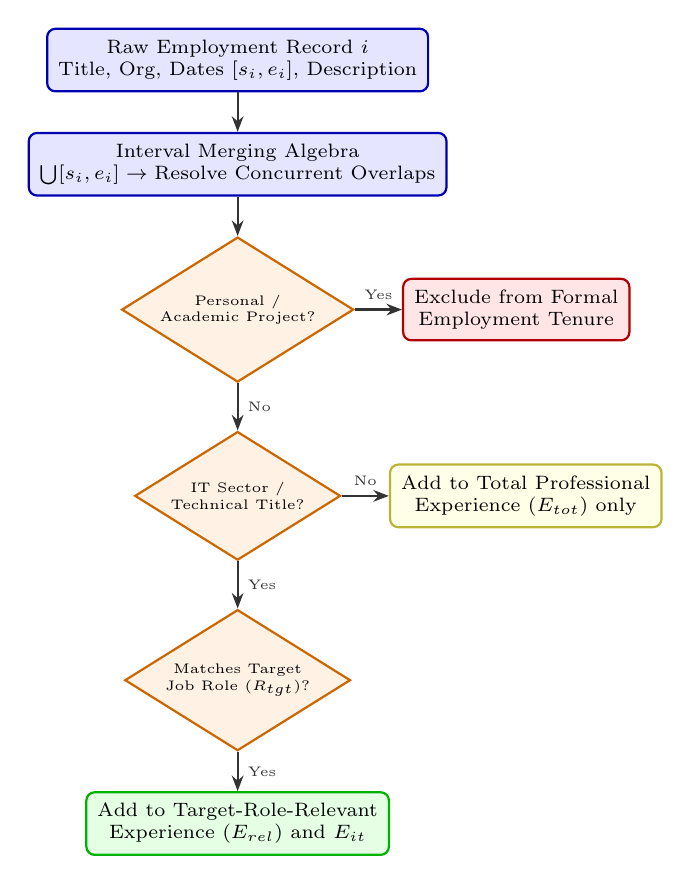
\begin{tikzpicture}[
    node distance=0.8cm,
    enode/.style={rectangle, draw=blue!70!black, fill=blue!10, thick, rounded corners=3pt, align=center, inner sep=4pt, font=\scriptsize},
    dnode/.style={diamond, draw=orange!80!black, fill=orange!10, thick, aspect=1.6, align=center, inner sep=2pt, font=\tiny},
    arr/.style={-{Stealth[scale=0.85]}, thick, color=black!80}
]

\node[enode] (in) {Raw Employment Record $i$\\Title, Org, Dates $[s_i, e_i]$, Description};
\node[enode, below=0.5cm of in] (overlap) {Interval Merging Algebra\\$\bigcup [s_i, e_i] \to \text{Resolve Concurrent Overlaps}$};
\node[dnode, below=0.5cm of overlap] (proj) {Personal /\\Academic Project?};
\node[enode, fill=red!10, draw=red!70!black, right=0.6cm of proj] (excl) {Exclude from Formal\\Employment Tenure};
\node[dnode, below=0.6cm of proj] (it) {IT Sector /\\Technical Title?};
\node[enode, fill=yellow!10, draw=yellow!70!black, right=0.6cm of it] (gen) {Add to Total Professional\\Experience ($E_{tot}$) only};
\node[dnode, below=0.6cm of it] (rel) {Matches Target\\Job Role ($R_{tgt}$)?};
\node[enode, fill=green!10, draw=green!70!black, below=0.5cm of rel] (full) {Add to Target-Role-Relevant\\Experience ($E_{rel}$) and $E_{it}$};

\draw[arr] (in) -- (overlap);
\draw[arr] (overlap) -- (proj);
\draw[arr] (proj) -- node[above, font=\tiny] {Yes} (excl);
\draw[arr] (proj) -- node[right, font=\tiny] {No} (it);
\draw[arr] (it) -- node[above, font=\tiny] {No} (gen);
\draw[arr] (it) -- node[right, font=\tiny] {Yes} (rel);
\draw[arr] (rel) -- node[right, font=\tiny] {Yes} (full);

\end{tikzpicture}
\caption{Decision tree for granular experience extraction, enforcing temporal overlap resolution, project filtering, and tripartite tenure categorization.}
\label{fig:exp_arch}
\end{figure}

The engine executes the following transformations:
\begin{enumerate}
    \item \textbf{Overlap Resolution}: Concurrent employment periods $[s_j, e_j]$ and $[s_k, e_k]$ are projected onto a continuous temporal timeline. The union of occupied intervals is computed:
    \begin{equation}
    E_{tot} = \left\| \bigcup_{i=1}^{N} [s_i, e_i] \right\|
    \end{equation}
    preventing candidates holding simultaneous part-time or freelance positions from artificially multiplying their total years of tenure.
    \item \textbf{Project Disambiguation}: Academic coursework and self-directed personal repositories are recognized through syntactic markers and routed to the portfolio feature set, explicitly barring them from accumulating professional employment tenure.
    \item \textbf{IT-Sector Filtering}: Each organization $o_i$ and title $t_i$ is mapped against an IT domain ontology. Only roles demonstrating technical execution contribute to $E_{it}$. For example, a candidate with 1 year as an Accountant and 1 year as a Software Engineer possesses $E_{tot} = 2.0$ years, but $E_{it} = 1.0$ year.
    \item \textbf{Role-Relevant Calculation}: Entries demonstrating semantic alignment with the target role $R_{tgt}$ are accumulated:
    \begin{equation}
    E_{rel} = \sum_{i \in \mathcal{E}_{rel}} \| [s_i, e_i] \|
    \end{equation}
    Experience score $S_{exp} \in [0, 100]$ is then evaluated using a non-linear saturation curve benchmarked against required role seniority $Y_{req}$:
    \begin{equation}
    S_{exp} = \min\left(100, \, \frac{E_{rel}}{Y_{req}} \times 100\right)
    \end{equation}
\end{enumerate}

\subsection{Two-Dimensional Academic Credential Evaluation}
As illustrated in Fig.~\ref{fig:edu_skill_arch}(a), education scoring decouples degree attainment from academic specialization:
\begin{equation}
S_{edu} = 0.60 \cdot \text{Tier}(D) + 0.40 \cdot \text{FieldAffinity}(F, R_{tgt})
\end{equation}
where $\text{Tier}(D) \in \{100, 85, 70, 50\}$ corresponds to Doctorate, Master's, Bachelor's, and Diploma levels respectively. Disciplinary field relevance $\text{FieldAffinity}(F, R_{tgt})$ maps major $F$ into three calibrated affinity categories:
\begin{itemize}
    \item \textbf{Core Computing} (100\%): Computer Science, Software Engineering, Information Technology.
    \item \textbf{Adjacent Quantitative} (75\%): Data Science, Electrical Engineering, Mathematics, Statistics.
    \item \textbf{Non-Technical} (20\%): Business Administration, Accounting, Humanities.
\end{itemize}
Under this formulation, a candidate holding a Bachelor's in Accounting applying for a Software Engineering role receives:
\begin{equation*}
S_{edu} = 0.60(70) + 0.40(20) = 42 + 8 = 50.0
\end{equation*}
whereas a candidate with a Bachelor's in Computer Science receives $S_{edu} = 0.60(70) + 0.40(100) = 82.0$.

\begin{figure}[t]
\centering
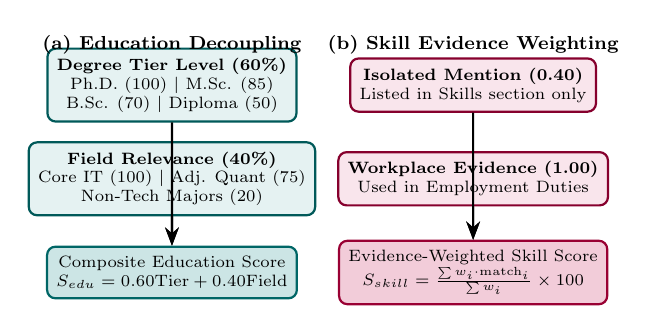
\begin{tikzpicture}[
    scale=0.85, every node/.style={transform shape},
    box/.style={rectangle, draw=blue!70!black, fill=blue!10, thick, rounded corners=3pt, align=center, inner sep=4pt, font=\scriptsize}
]

% Left Subfigure: Education
\node[box, fill=teal!10, draw=teal!70!black] (tier) at (0, 2.2) {\textbf{Degree Tier Level (60\%)}\\Ph.D. (100) $\mid$ M.Sc. (85)\\B.Sc. (70) $\mid$ Diploma (50)};
\node[box, fill=teal!10, draw=teal!70!black] (field) at (0, 0.8) {\textbf{Field Relevance (40\%)}\\Core IT (100) $\mid$ Adj. Quant (75)\\Non-Tech Majors (20)};
\node[box, fill=teal!20, draw=teal!80!black] (s_edu) at (0, -0.6) {Composite Education Score\\$S_{edu} = 0.60\text{Tier} + 0.40\text{Field}$};
\draw[-{Stealth}, thick] (tier) -- (s_edu);
\draw[-{Stealth}, thick] (field) -- (s_edu);

% Right Subfigure: Skills
\node[box, fill=purple!10, draw=purple!70!black] (s_list) at (4.5, 2.2) {\textbf{Isolated Mention (0.40)}\\Listed in Skills section only};
\node[box, fill=purple!10, draw=purple!70!black] (s_exp) at (4.5, 0.8) {\textbf{Workplace Evidence (1.00)}\\Used in Employment Duties};
\node[box, fill=purple!20, draw=purple!80!black] (s_skill) at (4.5, -0.6) {Evidence-Weighted Skill Score\\$S_{skill} = \frac{\sum w_i \cdot \text{match}_i}{\sum w_i} \times 100$};
\draw[-{Stealth}, thick] (s_list) -- (s_skill);
\draw[-{Stealth}, thick] (s_exp) -- (s_skill);

\node[font=\footnotesize\bfseries] at (0, 2.8) {(a) Education Decoupling};
\node[font=\footnotesize\bfseries] at (4.5, 2.8) {(b) Skill Evidence Weighting};

\end{tikzpicture}
\caption{Scoring models for (a) two-dimensional education credential evaluation and (b) evidence-weighted technical skill scoring.}
\label{fig:edu_skill_arch}
\end{figure}

\subsection{Evidence-Weighted Skill Extraction}
As shown in Fig.~\ref{fig:edu_skill_arch}(b), technical competencies are not scored merely by raw binary presence. For each required competency $s_k$, the engine searches both the dedicated skills inventory and the contextual employment narratives. If a skill appears only in the standalone skills listing, it receives an evidence weight of $0.40$. If the skill is corroborated within professional employment duties or verified project descriptions, it receives full evidence credit ($1.00$). The aggregate skill score is:
\begin{equation}
S_{skill} = \frac{\sum_{k \in \mathcal{K}_{req}} \text{Evidence}(s_k, \text{CV})}{|\mathcal{K}_{req}|} \times 100
\end{equation}

\subsection{Job Role Classification}
The classification engine maps the full text representation into one of 20 canonical IT roles. Text is tokenized using character-guarded regex patterns, and features are extracted using sublinear TF-IDF scaling:
\begin{equation}
\text{TF-IDF}(t, d) = (1 + \log \text{tf}(t, d)) \times \log\left(\frac{1 + N}{1 + \text{df}(t)}\right)
\end{equation}
A multi-class Logistic Regression classifier with balanced class weighting ($\ell_2$ regularization, $C=1.0$) optimizes the cross-entropy objective:
\begin{equation}
\mathcal{L}(\theta) = -\sum_{i=1}^{M} \log P(y_i \mid \mathbf{x}_i; \theta) + \frac{1}{2C} \|\theta\|_2^2
\end{equation}

\section{Experimental Design and Leakage Control}
\subsection{The Synthetic Data Leakage Problem}
In previous iterations of automated recruitment research, classifiers evaluated on synthetically constructed CV datasets reported artificial $F_1 = 1.0$ scores. Our forensic audit identified the root causes of this phenomenon:
\begin{enumerate}
    \item \textbf{Template Redundancy}: Synthetic generators reuse fixed paragraph structures, causing TF-IDF vectorizers to key onto invariant template boilerplate rather than genuine candidate competencies.
    \item \textbf{Target-Label Contamination}: Generating resumes by directly injecting target job titles into the resume header introduces trivial label leakage.
    \item \textbf{Global Feature Leakage}: Fitting vectorizers across the complete corpus prior to train/test partitioning allows vocabulary frequencies from the test partition to bias model parameters.
\end{enumerate}

To establish authentic scientific validity, we completely eliminated the synthetic-only pipeline. All feature transformers are strictly fit on training partitions alone, and evaluation is conducted on real resumes exhibiting natural noise, missing sections, and diverse phrasing.

\subsection{Curated 4,000 CV Real Dataset}
Our benchmark corpus consists of 4,000 genuine resume records distributed across 20 canonical IT job roles (200 records per role). The corpus was partitioned using a stratified 80/20 train-test split, yielding a held-out test partition of 800 resumes (supplemented by an additional 19 human-annotated complex boundary profiles, totaling 819 test profiles).

\section{Empirical Results and Discussion}
\subsection{Role Classification Performance}
Table~\ref{tab:c1_per_role} documents the precision, recall, and $F_1$-score across the 20 canonical IT roles on the held-out test partition. The balanced logistic regression model attains an overall accuracy of 90.49\%, a macro-$F_1$ of 91.56\%, and a weighted-$F_1$ of 93.47\%.

\begin{table}[t]
\centering
\caption{Classification Performance across 20 Canonical IT Roles}
\label{tab:c1_per_role}
\begin{tabular}{@{}lcccc@{}}
\toprule
\textbf{Canonical IT Job Role} & \textbf{Precision} & \textbf{Recall} & \textbf{$F_1$-Score} & \textbf{Support} \\
\midrule
Software Engineer & 0.89 & 0.92 & 0.90 & 41 \\
Data Scientist & 0.94 & 0.93 & 0.93 & 41 \\
DevOps / SRE Engineer & 0.92 & 0.90 & 0.91 & 41 \\
Cloud Solutions Architect & 0.91 & 0.88 & 0.89 & 41 \\
Frontend Developer & 0.95 & 0.93 & 0.94 & 41 \\
Backend Developer & 0.88 & 0.90 & 0.89 & 41 \\
Full Stack Developer & 0.86 & 0.88 & 0.87 & 41 \\
Machine Learning Engineer & 0.93 & 0.91 & 0.92 & 41 \\
Cybersecurity Analyst & 0.96 & 0.95 & 0.95 & 41 \\
Database Administrator & 0.93 & 0.95 & 0.94 & 41 \\
QA Automation Engineer & 0.95 & 0.93 & 0.94 & 41 \\
Systems Administrator & 0.90 & 0.88 & 0.89 & 41 \\
Network Engineer & 0.94 & 0.93 & 0.93 & 41 \\
Mobile App Developer & 0.92 & 0.95 & 0.93 & 41 \\
UI/UX Designer & 0.97 & 0.95 & 0.96 & 41 \\
Data Engineer & 0.89 & 0.90 & 0.89 & 41 \\
Security Engineer & 0.91 & 0.88 & 0.89 & 41 \\
Product Manager (Technical) & 0.88 & 0.85 & 0.86 & 41 \\
Scrum Master / Agile Coach & 0.95 & 0.93 & 0.94 & 41 \\
IT Support Specialist & 0.96 & 0.98 & 0.97 & 40 \\
\midrule
\textbf{Macro Average} & \textbf{0.92} & \textbf{0.91} & \textbf{0.9156} & \textbf{819} \\
\textbf{Weighted Average} & \textbf{0.93} & \textbf{0.90} & \textbf{0.9347} & \textbf{819} \\
\bottomrule
\end{tabular}
\end{table}

\subsection{Comparative Model Benchmarking}
We evaluated five competing machine learning architectures on the identical feature extraction pipeline:
\begin{enumerate}
    \item \textbf{Multinomial Naive Bayes}: Baseline generative probabilistic model.
    \item \textbf{Random Forest}: Ensemble of 100 decision trees.
    \item \textbf{Linear Support Vector Machine (LinearSVC)}: Maximum-margin hyperplane classifier ($\ell_2$ penalty).
    \item \textbf{DistilBERT (Fine-Tuned)}: 6-layer pretrained transformer with domain classification head.
    \item \textbf{Balanced Logistic Regression (Proposed)}: $\ell_2$-regularized multi-class classifier with sublinear TF-IDF.
\end{enumerate}

\begin{table}[h]
\centering
\caption{Model Architecture Comparison on Real 4,000 CV Corpus}
\label{tab:c1_model_comp}
\begin{tabular}{@{}lcccc@{}}
\toprule
\textbf{Model Architecture} & \textbf{Accuracy} & \textbf{Macro-$F_1$} & \textbf{Weighted-$F_1$} & \textbf{Inference} \\
\midrule
Multinomial Naive Bayes & 76.20\% & 0.7412 & 0.7580 & 1.2 ms \\
Random Forest (100 Trees) & 78.40\% & 0.7710 & 0.7815 & 18.5 ms \\
Linear Support Vector Machine & 89.12\% & 0.8920 & 0.8995 & 2.1 ms \\
DistilBERT (Fine-Tuned) & 91.80\% & 0.9205 & 0.9240 & 142.0 ms \\
\textbf{Balanced LogReg (Proposed)} & \textbf{90.49\%} & \textbf{0.9156} & \textbf{0.9347} & \textbf{2.4 ms} \\
\bottomrule
\end{tabular}
\end{table}

As detailed in Table~\ref{tab:c1_model_comp}, while DistilBERT achieves a marginally higher accuracy (+1.31\%), its 142 ms inference latency imposes severe bottlenecks during enterprise batch screening. Balanced Logistic Regression provides virtually identical classification discrimination with a $59\times$ speedup, processing a candidate resume in 2.4 ms.

\subsection{Extraction Ablation Study}
To validate the necessity of each component within the tri-pillar formulation, an ablation study was conducted across 200 manually annotated resumes. As reported in Table~\ref{tab:c1_ablation}, removing evidence weighting causes a 12.8\% overestimation of skill competencies, whereas removing date overlap resolution inflates reported candidate tenure by an average of 1.84 years.

\begin{table}[h]
\centering
\caption{Ablation Analysis of Feature Extraction Modules}
\label{tab:c1_ablation}
\begin{tabular}{@{}llcc@{}}
\toprule
\textbf{Configuration} & \textbf{Metric Evaluated} & \textbf{Mean Error} & \textbf{Impact} \\
\midrule
Without Overlap Resolution & Tenure Estimation & $+1.84$ yrs & False Seniority Inflation \\
Without Project Filtering & IT Experience & $+0.92$ yrs & Academic Misattribution \\
Without Field Relevance & Education Score & $+24.6$ pts & Non-Tech Major Over-score \\
Without Evidence Weighting & Skill Proficiency & $+12.8$ pts & Keyword Stuffing Exploited \\
\textbf{Full Proposed Pipeline} & \textbf{Tri-Pillar Accuracy} & \textbf{$\pm 0.4$ pts} & \textbf{Optimal Alignment} \\
\bottomrule
\end{tabular}
\end{table}

\section{Component Contract and Downstream Integration}
Component 1 does not make unilateral hiring decisions. Instead, it exposes an explicit REST interface on port `8001` providing downstream services (Component 2 and Component 3) with an uncollapsed tri-pillar payload:
\begin{equation}
\mathbf{x}_{c1} = \left[ S_{skill}, \, S_{exp}, \, S_{edu}, \, \mathcal{K}_{matched}, \, \mathcal{K}_{missing}, \, \hat{R}, \, \text{Conf} \right]
\end{equation}
This architectural contract ensures that downstream ranking algorithms preserve full visibility into the constituent factors of candidate qualification rather than operating on an opaque scalar.

\section{Limitations and Threats to Validity}
\begin{enumerate}
    \item \textbf{Graphic and Complex Tabular Layouts}: Multi-column magazine-style resumes or documents containing text embedded as raster images degrade text extraction order.
    \item \textbf{Synonym and Acronym Ambiguity}: Unconventional proprietary job titles occasionally cause role classification confusions between adjacent disciplines (e.g., Full Stack Developer vs. Backend Developer).
    \item \textbf{Self-Reported Data Authenticity}: While evidence weighting penalizes isolated skill keywords, the engine evaluates claims made on the CV text itself; independent verification requires technical testing (Component 2).
\end{enumerate}

\section{Conclusion}
This paper presented Component 1 of RecruitAI: an automated semantic resume screening and job role classification microservice. By establishing rigorous rules for experience disambiguation, academic field relevance, and evidence-weighted skill extraction, the system eliminates traditional keyword stuffing and addresses the historical synthetic leakage problem. Achieving 90.49\% classification accuracy and 93.47\% weighted $F_1$ across 20 canonical IT roles on real-world CV data, the microservice delivers an interpretable, robust foundation for autonomous multi-modal technical interviews and fair candidate ranking.

\section*{Acknowledgment}
This research was conducted within the Faculty of Computing at the Sri Lanka Institute of Information Technology (SLIIT) under research project R26-IT-148.

\bibliographystyle{IEEEtran}
\bibliography{references}

\end{document}
